\documentclass[a4paper]{article}

\usepackage[italian]{babel}
\usepackage[utf8]{inputenc}
\usepackage[T1]{fontenc}
\usepackage{enumitem}
\usepackage{graphicx}
\usepackage{float}
\usepackage{longtable}
\usepackage[table]{xcolor}
\usepackage{geometry}

\usepackage{lastpage}
\usepackage[bottom]{footmisc}
\usepackage{fancyhdr}
\usepackage{tabu}

\usepackage{pgffor}
\usepackage{etoolbox}
\usepackage{multirow}



\usepackage[official]{eurosym}

% Navigazione pdf
\usepackage{hyperref}
\hypersetup{
	colorlinks=true,
	linkcolor=black,
	filecolor=magenta,      
	urlcolor=blue,
}

\usepackage{tabularx}

\usepackage{multicol}
\newcommand{\glo}{\textsubscript{\emph{G}}}
\newcommand\hd{\emph{HD Viz}}
\newcommand\cod{\emph{Code of Duty}}
\newcommand{\myparagraph}[1]{\paragraph{#1}\mbox{}\\}
\newcommand{\mysubparagraph}[1]{\subparagraph{#1}\mbox{}\\}

\newcommand{\NdP}{\emph{Norme di Progetto 3.0.0}}
\newcommand{\PdP}{\emph{Piano di Progetto 3.0.0}}
\newcommand{\AdR}{\emph{Analisi dei requisiti 3.0.0}}
\newcommand{\PdQ}{\emph{Piano di Qualifica 3.0.0}}

\definecolor{header}{HTML}{FA8D21}
\definecolor{pari}{HTML}{DBDBDB}
\definecolor{dispari}{HTML}{F5F5F5}

\setcounter{secnumdepth}{4}

\pagestyle{fancy}
\lhead{
\includegraphics[scale=0.06]{../_template/images/logo_crop.png}}

%Titolo del documento
\rhead{\titolodocumento{}}
\cfoot{Pagina \thepage\ di \pageref{LastPage}}
\renewcommand{\footrulewidth}{0.4pt}

\newcommand{\titolodocumento}{Analisi dei requisiti} % Titolo documento
\newcommand{\versione}{ 2.3.0 } % Versione documento
\newcommand{\approvazione}{ Diego Piola } % Responsabile di progetto
\newcommand{\redazione}{\parbox[t]{4cm} {Andrea Mascari\\Damiano Zanardo\\Diego Piola\\}} % Redattori di questo documento
\newcommand{\verifica}{\parbox[t]{4cm} {Andrea Mascari\\Damiano Zanardo \\ Diego Piola \\ Alessandro Flori \\ } } % Verificatori di questo documento
\newcommand{\stato}{In lavorazione} % Approvato 
\newcommand{\uso}{Esterno} % Interno - Esterno
\newcommand{\destinazione}{\parbox[t]{4cm}{Prof Tullio Vardanega \\ Prof. Riccardo Cardin} } % Destinatario ( D1\\D2\\D3 )
\newcommand{\descrizionedocumento}{Il documento elenca casi d'uso e requisiti del progetto } % Descrizione documento

% Mettere sempre la virgola dopo l'ultima riga, se no si rompe la tabella

\def\modifiche{
    {v0.0.1, 02/12/2020, Damiano Zanardo, Analista , Prima bozza{,} aggiunti tutti i capitolati},
}



% Per modificare il frontespizio e diario delle modifiche andare sulla cartella source
% Per aggiungere il contenuto andare sulla cartella source/sections e creare un nuovo file.tex per ogni sezione

% Per parole che devono andare nel glossario aggiungere /glo{} dopo la parola
\begin{document}
    % Frontespizio 
    %\documentclass[a4paper]{article}
%\usepackage[italian]{babel}
\usepackage[utf8]{inputenc}
\usepackage[T1]{fontenc}
\usepackage{enumitem}
\usepackage{graphicx}
\usepackage{float}
\usepackage{longtable}
\usepackage[table]{xcolor}
\usepackage{geometry}

\usepackage{lastpage}
\usepackage[bottom]{footmisc}
\usepackage{fancyhdr}
\usepackage{tabu}

\usepackage{pgffor}
\usepackage{etoolbox}
\usepackage{multirow}



\usepackage[official]{eurosym}

% Navigazione pdf
\usepackage{hyperref}
\hypersetup{
	colorlinks=true,
	linkcolor=black,
	filecolor=magenta,      
	urlcolor=blue,
}

\usepackage{tabularx}

\usepackage{multicol}
%\begin{document}

\begin{titlepage}

	\begin{center}
		
\includegraphics[scale = 0.5]{../_template/images/logo.png}\\
		\large \textbf{Code of Duty - Progetto \emph{HD VIZ}} \\
		\vfill
		\huge \textbf{\titolodocumento}
		\vspace*{\fill}
        
        \vfill
        \large
    \end{center}
    
	\begin{table}[htbp]
        \centering
        \begin{tabular}{r|l}
            \textbf{Versione} & \versione{} \\
            \textbf{Approvazione} & \approvazione{} \\
            \textbf{Redazione} & \redazione{} \\
            \textbf{Verifica} & \verifica{} \\
            \textbf{Stato} & \stato{} \\
            \textbf{Uso} & \uso{} \\
            \textbf{Destinato a} & \destinazione{}
        \end{tabular}
    \end{table}
    
    \begin{center}
        \vfill
        \normalsize
        \textbf{Descrizione}\\
		\descrizionedocumento
        \vfill
        \small
        \texttt{info@codeofduty.it}
	\end{center}
\end{titlepage}

%\end{document}

    
    % Diario delle modifiche
    \newcommand*\mytablecontents{}
\foreach \x [count=\nj] in \modifiche
{
    \foreach \y [count=\ni] in \x
    {
        \ifnum\ni=6
            \xappto\mytablecontents{\y}
            \gappto\mytablecontents{\\}
            \gappto\mytablecontents{\hline}
        \else
            \xappto\mytablecontents{\y&}
        \fi
    }
}

\section*{Diario delle modifiche}

% Impostazioni della tabella
\tabulinesep = 2mm % padding
\taburowcolors [1] 2{pari .. dispari} % colori delle righe
\begin{longtabu} to \textwidth {| X[0.3, c m] | X[0.6,c m] | X[0.7,c m] | X[0.9,c m] | X[0.7,c m] | X[1.2,l m]|} % larghezza delle colonne
\hline
\rowcolor{header} % colore dell'header

\textbf{Ver.} & \textbf{Data} & \textbf{Nominativo} & \textbf{Ruolo} & \textbf{Verificatore} & \multicolumn{1}{c|}{\textbf{Descrizione}}\\
\hline
\mytablecontents

\end{longtabu}

    \pagebreak
    
    % Indice
    \tableofcontents
    \pagebreak
    
    % Se necessari
    % \listoffigures
    % \listoftables
    
    % Contenuto

    \section{Introduzione}
\subsection{Scopo del documento}
	In questo documento vengono illustrate le modalità con cui il gruppo \textit{Code of Duty} affronterà lo sviluppo del progetto \hd, quali:
	\begin{itemize}
    		\item Analisi dei rischi;
    		\item Presentazione del modello di sviluppo adottato;
    		\item Pianificazione delle attività e divisione dei ruoli;
    		\item Stima dei costi economici e risorse necessarie al compimento del progetto.
	\end{itemize}
\subsection{Scopo del prodotto}
	L'obiettivo del progetto è quello di creare un'applicazione di visualizzazione di dati con molte dimensioni. L'applicazione dovra permettere diverse visualizzazioni dei dati tramite browser ed è richiesta anche una parte server di supporto che permetta il prelevamento dei dati e la loro elaborazione.
\subsection{Glossario}
	In questo documento vengono definiti e descritti tutti i termini e tecnologie al fine di evitare ambiguità relative al linguaggio utilizzato nei documenti formali. Per facilitare la lettura i termini saranno contrassegnati da una 'G' a pedice.  
\subsection{Riferimenti}
	\subsubsection{Normativi}
		\begin{itemize}
			\item \textbf{Norme di Progetto}: \textit{Norme di progetto 2.0.0};
			\item \textbf{Regolamento organigramma e specifica tecnico-economica} : \href{https://www.math.unipd.it/~tullio/IS-1/2020/Progetto/RO.html}{RO}.
		\end{itemize}
	\subsubsection{Informativi}
		\begin{itemize}
			\item \textbf{Capitolato d'interesse}: \href{https://www.math.unipd.it/~tullio/IS-1/2020/Progetto/C4.pdf}{HD Viz - Visualizzazione di dati con molte dimensioni};
			\item \textbf{Il ciclo di vita del Software}: \href{https://www.math.unipd.it/~tullio/IS-1/2020/Dispense/L05.pdf}{L05};
			\item \textbf{Gestione di progetto}: \href{https://www.math.unipd.it/~tullio/IS-1/2020/Dispense/L06.pdf}{L06}.
		\end{itemize}
\subsection{Scadenze}
	Il gruppo \textit{Code of Duty} ha deciso di impegnarsi a rispettare le seguenti scadenze per lo sviluppo del progetto \hd
	\begin{itemize}
		\item \textbf{Revisione dei Requisiti}: 11-Gennaio-2021;
		\item \textbf{Revisione di Progettazione}: 10-Marzo-2021;
		\item \textbf{Revisione di Qualifica}: 2-Aprile-2021;
		\item \textbf{Revisione di Accettazione}: 3-Maggio-2021;
	\end{itemize}

    \newpage
    \section{Qualità di processo}
Per ottenere la più alta qualità delle attività e processi, e per rientrare nelle tempistiche stipulate nel Piano di progetto, verrà analizzato ed applicato l' ISO/IEC/IEEE 12207:1995.

Sono stati scelti quindi i processi ritenuti più adeguati ed attinenti al progetto i quail sono stati divisi in due categorie: primari e di supporto. Verrano di seguito riportate i processi appartenenti a tali categorie, e i loro obiettivi e metriche in modo da ottenere una qualità quantificabile.
    \subsection{Processi primari}
        \subsubsection{Fornitura}
            \paragraph{Obiettivi}
            \paragraph{Metriche}
            
        \subsubsection{Pianificazione}
        L'attività di pianificazione ingloba il monitoramento delle risorse quali i tempi a disposizione i costi e la divisione dei ruoli e la loro distribuzione.La scelta di mettere la Pianificazione come processo primario è data dalla sua importanza nel progetto. Inoltre viene esposta maggiormente all'interno del documento Piano di progetto.
            \paragraph{Strategie e Obiettivi}
                \begin{itemize}
                    \item \textbf{Costi}: analizzare e quantificare costi e tempistiche
                    \item \textbf{Metriche}: per fare in modo che i  tali costi non si discostino più di un margine prescelto devono essere usate le metriche scelte.
                    \item \textbf{Calendarizzazione}: per assicurare che le tempistiche dello svolgimento del progetto siano adeguate bisogna seguire le direttive della calendarizzazione del progetto
                    \item \textbf{Aggiornamenti}: mantenere aggiornato il gruppo ed i verbali durante tutti il progetto in modo da quantificare il cambiamento delle risorse
                \end{itemize}
                
           \paragraph{Metriche}
           alcunee metriche per la pianificazione sono usate per calcolarne delle altre e la loro formula è semplicemente data dal volre intero che hanno
            \def\productquality{
            {   , 
                Budget at Completion,
                numero intero, 
                $ \pm 5 \% $ del preventivo,
                pari al preventivo
            },
            {   , 
                Earned value,
                BAC - $\%$ di lavoro completato, 
                $ >0$,
                $ >0$
            },
            {   , 
                Planned value,
                valore pianificato nel momento del calcolo, 
                $ >0$,
                $ >0$
            },
            {   , 
                Acual cost,
               numero intero, 
                0 < AC $\leq$ budget totale,
                0 < AC $\leq$ PV
            },
            {   , 
                Schedule variance,
               SV = EV - PV, 
                $ >0$,
                $ 0$
            },
            {   , 
                Cost variance,
               CV = EV - AC, 
                $ >0$,
                $ \geq 0$
            },
        }
 \newcommand*\metricstable{}
\foreach \x [count=\nj] in \productquality
{
    \foreach \y [count=\ni] in \x
    {
        \ifnum\ni=5
            \xappto\metricstable{\y}
            \gappto\metricstable{\\}
            \gappto\metricstable{\hline}
        \else\ifnum\ni=6
            \xappto\metricstable{\noexpand\multicolumn{5}{| l |}{NOTE: \y}}
            \gappto\metricstable{\\}
            \gappto\metricstable{\hline}
        \else
            \xappto\metricstable{\y&}
        \fi\fi
    }
}

% Impostazioni della tabella
\tabulinesep = 2mm % padding
\taburowcolors [1] 2{pari .. dispari} % colori delle righe
\begin{longtabu} to \textwidth {| X[0.5, c m] | X[0.6,c m] | X[0.9,c m] | X[0.8,c m] | X[1.2,c m]|} % larghezza delle colonne
\hline
\rowcolor{header} % colore dell'header

\textbf{Codice} & \textbf{Nome} & \textbf{Formula} & \textbf{Valore sufficiente} & \textbf{Valore ottimo}\\
\hline
\metricstable

\end{longtabu}

\undef\metricstable{}



        
    \subsubsection{Sviluppo}
        
        \subsection{Processi di supporto}
            \subsubsection{Documentazione}
            \subsubsection{Quality assurance}
            \subsubsection{Verification process}

    \newpage
    \section{Qualità di Prodotto}
In questa sezione sono indicati valori sufficienti e ottimi delle metriche individuate e descritte nelle Norme di Progetto.
In particolare una misurazione di qualità per essere considerata soddisfatta deve essere superiore al valore sufficiente indicato. 
Il valore ottimo individua un obiettivo di qualità da raggiungere o mantenere per l'intera durata dell'attività di progetto.
\subsection{ISO 9126}
Per la Qualità di Prodotto il team ha deciso di seguire i principi di ISO 9126.
Lo Standard definisce 6 caratteristiche di qualità che deve possedere un prodotto: funzionalità, affidabilità, efficienza, usabilità, manutenibilità e portabilità. 
Non sono state individuate metriche di portabilità in quanto è stata considerata una caratteristica non rilevante nel prodotto sviluppato. 
ISO 9126 oltre a 6 caratteristiche individua 3 tipologie di misurazioni: della qualità interna, esterna e qualità in uso. 
In questa sezione non è tenuto conto della distinzione e non sono presenti metriche di qualità in uso, che richiedono necessariamente l'utilizzo del prodotto da parte di un utente.

\subsection{Funzionalità}
\def\productquality{
    {   , 
        Correttezza dello scambio dei dati,
        $N_{err}$, 
        -,
        0
    },
}
\newcommand*\metricstable{}
\foreach \x [count=\nj] in \productquality
{
    \foreach \y [count=\ni] in \x
    {
        \ifnum\ni=5
            \xappto\metricstable{\y}
            \gappto\metricstable{\\}
            \gappto\metricstable{\hline}
        \else\ifnum\ni=6
            \xappto\metricstable{\noexpand\multicolumn{5}{| l |}{NOTE: \y}}
            \gappto\metricstable{\\}
            \gappto\metricstable{\hline}
        \else
            \xappto\metricstable{\y&}
        \fi\fi
    }
}

% Impostazioni della tabella
\tabulinesep = 2mm % padding
\taburowcolors [1] 2{pari .. dispari} % colori delle righe
\begin{longtabu} to \textwidth {| X[0.5, c m] | X[0.6,c m] | X[0.9,c m] | X[0.8,c m] | X[1.2,c m]|} % larghezza delle colonne
\hline
\rowcolor{header} % colore dell'header

\textbf{Codice} & \textbf{Nome} & \textbf{Formula} & \textbf{Valore sufficiente} & \textbf{Valore ottimo}\\
\hline
\metricstable

\end{longtabu}

\undef\metricstable{}


\subsection{Affidabilità}
\def\productquality{
    {   , 
        Densità di errori,
        $N_{err}/SLOC$, 
        -,
        -,
        è stato ritenuto prematuro definire valori sufficienti e ottimi per la metrica
    },
}
\newcommand*\metricstable{}
\foreach \x [count=\nj] in \productquality
{
    \foreach \y [count=\ni] in \x
    {
        \ifnum\ni=5
            \xappto\metricstable{\y}
            \gappto\metricstable{\\}
            \gappto\metricstable{\hline}
        \else\ifnum\ni=6
            \xappto\metricstable{\noexpand\multicolumn{5}{| l |}{NOTE: \y}}
            \gappto\metricstable{\\}
            \gappto\metricstable{\hline}
        \else
            \xappto\metricstable{\y&}
        \fi\fi
    }
}

% Impostazioni della tabella
\tabulinesep = 2mm % padding
\taburowcolors [1] 2{pari .. dispari} % colori delle righe
\begin{longtabu} to \textwidth {| X[0.5, c m] | X[0.6,c m] | X[0.9,c m] | X[0.8,c m] | X[1.2,c m]|} % larghezza delle colonne
\hline
\rowcolor{header} % colore dell'header

\textbf{Codice} & \textbf{Nome} & \textbf{Formula} & \textbf{Valore sufficiente} & \textbf{Valore ottimo}\\
\hline
\metricstable

\end{longtabu}

\undef\metricstable{}


\subsection{Efficienza}


\subsection{Usabilità}


\subsection{Manutenibilità}

    \section{Specifica dei test}

Sono stati determinati, come descritto anche nel documento \NdP , 5 tipi di test ovvero: 
\textit{Test di unità, Test di Integrazione, Test di sistema, Test di accettazione} e \textit{Test di regressione}. 
Si adotterà quindi il \textbf{Modello a V} che permette lo sviluppo dei test in parallelo alle attività di analisi e progettazione. 
Così facendo i test sviluppati saranno in grado di verificare sia la correttezza del programma software sia l'implementazione. 
Sara disponibile inoltre una tabella degli esiti dei test per una facile consultazione.
Per i test valgono le seguenti sigle:

    \begin{itemize}
        \item \textbf{S}: il test è stato implementato e ha esito soddisfacente.
        \item \textbf{NS}: il test è stato implementato e non ha esito soddisfacente.
        \item \textbf{NI}: per indicare che il test è ancora non implementato.
    \end{itemize}
 
\subsection{Test di Sistema}
Per rispettare i requisiti identificati nel documento \AdR\ e per garantire il funzionamento del prodotto si eseguono i seguenti Test di sistema:\\
    
\subsubsection{Test di sistema per i requisiti funzionali}
    \hphantom{}

    %startTable
    \def\testspecification{
    {   
        TSOF1,
        Si verifica che l'utente possa caricare i dati per la visualizzazione tramite file CSV,
        S,
        RFO1 RFO1.1
    },
    {   
        TSOF1.1,
        Si verifica che l'utente possa inserire i dati tramite query al database,
        S,
        RFO1.2
    },
    {   
        TSOF1.2,
        Si verifica che appaia un messaggio d'errore in caso di errore nell'inserimento dei dati,
        S,
        RFO1.3
    },
    {   
        TSOF1.3,
        Si verifica che i dati caricati provenienti da qualsiasi fonte siano convertiti in JSON,
        S,
        RFO1.4
    },
    {   
        TSOF2,
        Si verifica la possibilità di scelta nella visualizzazione dei dati. In particolare devono essere presenti le seguenti visualizzazioni:
        \unexpanded{
        \begin{itemize}
            \item Scatter Plot Matrix
            \item Heatmap
            \item Force Field
            \item Linear Projection
        \end{itemize}},
        S,
        RFO2 RFO2.1 RFO2.2 RFO2.4 RFO2.5
    },
    {   
        TSFF2.1,
        Si verifica che nella scelta per la visualizzazione deve esserci: Correlation Heatmap,
        S,
        RFF2.3
    },
    {   
        TSFF2.2,
        Si verifica che nella scelta per la visualizzazione deve esserci: Parallel Coordinates,
        S,
        RFF2.6
    },
    {   
        TSOF3,
        Si verifica che l'utente possa manipolare i dati nel dataset,
        S,
        RFO3
    },
    {   
        TSOF3.1,
        SI verifica che l'utente possa selezionare le variabili target tra le features del dataset,
        S,
        RFO3.1
    },
    {   
        TSOF3.2,
        SI verifica che l'utente possa selezionare le features a cui è interessato,
        S,
        RFO3.2
    },
    {   
        TSOF3.3,
        SI verifica che l'utente possa normalizzare i dati presenti nel dataset nei seguenti modi:
        \unexpanded{
        \begin{itemize}
            \item Globalmente
            \item Per colonna
        \end{itemize}},
        S,
        RFO3.3 RFO3.3.1 RFO 3.3.2 RFO 3.3.3
    },
    {   
        TSFF3.4,
        SI verifica che l'utente possa selezionare le righe del dataset a cui è interessato,
        S,
        RFF3.4
    },
    {   
        TSOF4,
        Si verifica che l'utente possa modificare le impostazioni che influenzano la visualizzazione,
        S,
        RFO4
    },
    {   
        TSOF4.1,
        Si verifica che l'utente possa assegnare una classe di visualizzazione ad ogni variabile target selezionata,
        S,
        RFO4.1
    },
    {   
        TSOF4.2,
        Si verifica che l'utente possa modificare il range dei dati da considerare nella Heatmap,
        S,
        RFO4.2
    },
    {   
        TSOF4.3,
        Si verifica che l'utente possa assegnare un colore al range di un Heatmap,
        S,
        RFO4.3
    },
    {   
        TSOF4.4,
        Si verifica che l'utente che ha selezionato la visualizzazione Heatmap possa ordinare in ordine alfabetico e in cluster il dataset,
        S,
        RFO4.4 RFO4.4.1 RFO4.4.2
    },
    {   
        TSOF5,
        Si verifica che l'utente possa calcolare la matrice di distanza se ha scelto la visualizzazione Heatmap o Forcefield,
        S,
        RFO5
    },    
    {   
        TSOF5.1,
        Si verifica che siano disponibili i seguenti tipi di distanze per calcolare la matrice di distanza:
        \unexpanded{
            \begin{itemize}
                \item euclidea;
                \item Manhattan.
            \end{itemize}
        }
        E che siano disponibili per Forcefield e Heatmap,
        S,
        RFO5.1 RFO5.1.1 RFO5.1.2
    },
    {   
        TSOF6,
        Si verifica che quando viene scelta la visualizzazione Linear Projection sia calcolata la riduzione delle componenti,
        S,
        RFO6
    },
    {   
        TSFF6.1,
        Si verifica che l'utente possa scegliere tra i seguenti algoritmi per la riduzione dei componenti:
        \unexpanded{
        \begin{itemize}
            \item PCA;
            \item UMAP;
            \item t-SNE.
        \end{itemize}},
        S,
        RFO6.1 RFF6.1.1 RFF6.1.2 6.1.3
    },
    {   
        TSOF7,
        Si verifica che la visualizzazione creata dal sistema sia salvabile in formato PNG,
        S,
        RFO7
    },
    {   
        TSOF8,
        Si verifica che un messaggio di errore compaia a schermo se i file sono caricati scorrettamente,
        S,
        RFO8
    },
    }
    \newcommand*\testdescription{}
\foreach \x [count=\nj] in \testspecification
{
    \foreach \y [count=\ni] in \x
    {
        \ifnum\ni=4
            \xappto\testdescription{\y}
            \gappto\testdescription{\\}
            \gappto\testdescription{\hline}
        \else
            \xappto\testdescription{\y&}
        \fi
    }
}

% Impostazioni della tabella
\tabulinesep = 2mm % padding
\taburowcolors [1] 2{pari .. dispari} % colori delle righe
\begin{longtabu} to \textwidth {| X[0.1,c m] | X[0.2,c m] | X[0.1,c m] | X[0.1,c m]|} % larghezza delle colonne
\hline
\rowcolor{header} % colore dell'header

\textbf{ID test} & \textbf{Descrizione} & \textbf{Esito} & \textbf{ID requisito} \\
\hline
\testdescription

\end{longtabu}

\undef\testdescription{}

    %endTable
    
\subsubsection{Test di sistema per i requisiti di qualità}
    %startTable
    \def\testspecification{
    {   
        TSOQ1,
        Si verifica che sia stato prodotto un manuale d'uso per l'utente,
        S,
        RQO1
    },
    {   
        TSOQ2,
        Si verifica che sia stato prodotto un manuale manutentore,
        S,
        RQO2
    },
    {   
        TSOQ3,
        Si verifica che il codice sia stato pubblicato su un repository pubblico,
        S,
        RQO3
    },
    {   
        TSOQ4,
        Si verifica che il codice segua le norme di stile specificate nel documento Norme di Progetto,
        S,
        RQO4
    },
    {   
        TSOQ5,
        Si verifica che nella codifica si eviti l'utilizzo di chiamate ricorsive dove è possibile,
        S,
        RQO5
    },
      }
    \newcommand*\testdescription{}
\foreach \x [count=\nj] in \testspecification
{
    \foreach \y [count=\ni] in \x
    {
        \ifnum\ni=4
            \xappto\testdescription{\y}
            \gappto\testdescription{\\}
            \gappto\testdescription{\hline}
        \else
            \xappto\testdescription{\y&}
        \fi
    }
}

% Impostazioni della tabella
\tabulinesep = 2mm % padding
\taburowcolors [1] 2{pari .. dispari} % colori delle righe
\begin{longtabu} to \textwidth {| X[0.1,c m] | X[0.2,c m] | X[0.1,c m] | X[0.1,c m]|} % larghezza delle colonne
\hline
\rowcolor{header} % colore dell'header

\textbf{ID test} & \textbf{Descrizione} & \textbf{Esito} & \textbf{ID requisito} \\
\hline
\testdescription

\end{longtabu}

\undef\testdescription{}

    %endTable  
        
\subsubsection{Test di sistema per i requisiti di vincolo}
    %startTable
    \def\testspecification{
    {   
        TSOV1,
        Si verifica che il codice sorgente dell'applicazione sia open source,
        S,
        RVO1
    },
    {   
        TSOV2,
        Si verifica che l'applicazione sia sviluppata in Javascript con l'utilizzo della libreria d3.js,
        S,
        RVD2 RVD2.1
    },
    {   
        TSDV2.1,
        Si verifica che il backend dell'applicazione sia sviluppato con node.js con l'utilizzo del framework Express,
        S,
        RVD2.2
    },
    {   
        TSDV2.2,
        Si verifica che il frontend dell'applicazione sia sviluppato con React con l'utilizzo del framework Ant Design,
        S,
        RVD2.3
    },
    {   
        TSOV3,
        Si verifica che i dati siano convertibili in JSON,
        S,
        RVO3
    },
    {   
        TSOV4,
        Si verifica che nella visualizzazione Scatter Plot Matrix si possano visualizzare al massimo 5 features,
        S,
        RVO4
    },
    {   
        TSDV5,
        Si verifica che la libreria per PCA sia ml-pca,
        S,
        RVD5
    },
    {   
        TSDV6,
        Si verifica che la libreria per Umap sia tsne-js,
        S,
        RVD6
    },
    {   
        TSDV7,
        Si verifica che la libreria per t-SNE sia tsne-js,
        S,
        RVD7
    },
    {   
        TSDV8,
        Si verifica che la libreria per le distanze sia ml-distance,
        S,
        RVD8
    },
    {   
        TSDV9,
        Si verifica che la libreria per la matrice di correlazione sia jeezy,
        S,
        RVD9
    },
      }
    \newcommand*\testdescription{}
\foreach \x [count=\nj] in \testspecification
{
    \foreach \y [count=\ni] in \x
    {
        \ifnum\ni=4
            \xappto\testdescription{\y}
            \gappto\testdescription{\\}
            \gappto\testdescription{\hline}
        \else
            \xappto\testdescription{\y&}
        \fi
    }
}

% Impostazioni della tabella
\tabulinesep = 2mm % padding
\taburowcolors [1] 2{pari .. dispari} % colori delle righe
\begin{longtabu} to \textwidth {| X[0.1,c m] | X[0.2,c m] | X[0.1,c m] | X[0.1,c m]|} % larghezza delle colonne
\hline
\rowcolor{header} % colore dell'header

\textbf{ID test} & \textbf{Descrizione} & \textbf{Esito} & \textbf{ID requisito} \\
\hline
\testdescription

\end{longtabu}

\undef\testdescription{}

    %endTable
     
\subsection{Test di accettazione}
    \subsubsection{Test di accettazione per i requisiti funzionali}
        \hphantom{}
        %startTable
        \def\testspecification{
        {   
            TAOF1,
            Si verifica che l'utente possa caricare i dati per la visualizzazione tramite file CSV,
            S,
            RFO1 RFO1.1
        },
        {   
            TAOF1.1,
            Si verifica che l'utente possa inserire i dati tramite query al database,
            S,
            RFO1.2
        },
        {   
            TAOF1.2,
            Si verifica che appaia un messaggio d'errore in caso di errore nell'inserimento dei dati,
            S,
            RFO1.3
        },
        {   
            TAOF1.3,
            Si verifica che i dati caricati provenienti da qualsiasi fonte siano convertiti in JSON,
            S,
            RFO1.4
        },
        {   
            TAOF2,
            Si verifica la possibilità di scelta nella visualizzazione dei dati. In particolare devono essere presenti le seguenti visualizzazioni:
            \unexpanded{
            \begin{itemize}
                \item Scatter Plot Matrix
                \item Heatmap
                \item Force Field
                \item Linear Projection
            \end{itemize}},
            S,
            RFO2 RFO2.1 RFO2.2 RFO2.4 RFO2.5
        },
        {   
            TAOF3,
            Si verifica che l'utente possa manipolare i dati nel dataset,
            S,
            RFO3
        },
        {   
            TAOF3.1,
            SI verifica che l'utente possa selezionare le variabili target tra le features del dataset,
            S,
            RFO3.1
        },
        {   
            TAOF3.2,
            SI verifica che l'utente possa selezionare le features a cui è interessato,
            S,
            RFO3.2
        },
        {   
            TAOF3.3,
            SI verifica che l'utente possa normalizzare i dati presenti nel dataset nei seguenti modi:
            \unexpanded{
            \begin{itemize}
                \item Globalmente
                \item Per colonna
            \end{itemize}},
            S,
            RFO3.3 RFO3.3.1 RFO3.3.2 RFO3.3.3
        },
        {   
            TAOF4,
            Si verifica che l'utente possa modificare le impostazioni che influenzano la visualizzazione,
            S,
            RFO4
        },
        {   
            TAOF4.1,
            Si verifica che l'utente possa assegnare una classe di visualizzazione ad ogni variabile target selezionata,
            S,
            RFO4.1
        },
        {   
            TAOF4.2,
            Si verifica che l'utente possa modificare il range dei dati da considerare nella Heatmap,
            S,
            RFO4.2
        },
        {   
            TAOF4.3,
            Si verifica che l'utente possa assegnare un colore al range di un Heatmap,
            S,
            RFO4.3
        },
        {   
            TAOF4.4,
            Si verifica che l'utente che ha selezionato la visualizzazione Heatmap possa ordinare in ordine alfabetico e in cluster il dataset,
            S,
            RFO4.4 RFO4.4.1 RFO4.4.2
        },
        {   
            TAOF5,
            Si verifica che l'utente possa calcolare la matrice di distanza se ha scelto la visualizzazione Heatmap o Forcefield,
            S,
            RFO5
        },    
        {   
            TAOF5.1,
            Si verifica che siano disponibili i seguenti tipi di distanze per calcolare la matrice di distanza:
            \unexpanded{
                \begin{itemize}
                    \item euclidea;
                    \item Manhattan.
                \end{itemize}
            }
            E che siano disponibili per Forcefield e Heatmap,
            S,
            RFO5.1 RFO5.1.1 RFO5.1.2
        },
        {   
            TAOF6,
            Si verifica che quando viene scelta la visualizzazione Linear Projection sia calcolata la riduzione delle componenti,
            S,
            RFO6
        },
        {   
            TAFF6.1,
            Si verifica che l'utente possa scegliere tra i seguenti algoritmi per la riduzione dei componenti:
            \unexpanded{
            \begin{itemize}
                \item PCA;
                \item UMAP;
                \item t-SNE.
            \end{itemize}}
            Due o più di questi algoritmi devono essere implementati,
            S,
            RFO6.1 RFF6.1.1 RFF6.1.2 6.1.3
        },
        {   
            TAOF7,
            Si verifica che la visualizzazione creata dal sistema sia salvabile in formato PNG,
            S,
            RFO7
        },
        {   
            TAOF8,
            Si verifica che un messaggio di errore compaia a schermo se i file sono caricati scorrettamente,
            S,
            RFO8
        },
        }
        \newcommand*\testdescription{}
\foreach \x [count=\nj] in \testspecification
{
    \foreach \y [count=\ni] in \x
    {
        \ifnum\ni=4
            \xappto\testdescription{\y}
            \gappto\testdescription{\\}
            \gappto\testdescription{\hline}
        \else
            \xappto\testdescription{\y&}
        \fi
    }
}

% Impostazioni della tabella
\tabulinesep = 2mm % padding
\taburowcolors [1] 2{pari .. dispari} % colori delle righe
\begin{longtabu} to \textwidth {| X[0.1,c m] | X[0.2,c m] | X[0.1,c m] | X[0.1,c m]|} % larghezza delle colonne
\hline
\rowcolor{header} % colore dell'header

\textbf{ID test} & \textbf{Descrizione} & \textbf{Esito} & \textbf{ID requisito} \\
\hline
\testdescription

\end{longtabu}

\undef\testdescription{}

        %endTable
    \subsubsection{Test di accettazione per i requisiti di qualità}
        %startTable
        \def\testspecification{
            {   
                TAOQ1,
                Si verifica che sia stato prodotto un manuale d'uso per l'utente,
                S,
                RQO1
            },
            {   
                TAOQ2,
                Si verifica che sia stato prodotto un manuale manutentore,
                S,
                RQO2
            },
            {   
                TAOQ3,
                Si verifica che il codice sia stato pubblicato su un repository pubblico,
                S,
                RQO3
            },
        }
        \newcommand*\testdescription{}
\foreach \x [count=\nj] in \testspecification
{
    \foreach \y [count=\ni] in \x
    {
        \ifnum\ni=4
            \xappto\testdescription{\y}
            \gappto\testdescription{\\}
            \gappto\testdescription{\hline}
        \else
            \xappto\testdescription{\y&}
        \fi
    }
}

% Impostazioni della tabella
\tabulinesep = 2mm % padding
\taburowcolors [1] 2{pari .. dispari} % colori delle righe
\begin{longtabu} to \textwidth {| X[0.1,c m] | X[0.2,c m] | X[0.1,c m] | X[0.1,c m]|} % larghezza delle colonne
\hline
\rowcolor{header} % colore dell'header

\textbf{ID test} & \textbf{Descrizione} & \textbf{Esito} & \textbf{ID requisito} \\
\hline
\testdescription

\end{longtabu}

\undef\testdescription{}

        %endTable  
            
    \subsubsection{Test di accettazione per i requisiti di vincolo}
        %startTable
        \def\testspecification{
            {   
                TAOV1,
                Si verifica che il codice sorgente dell'applicazione sia open source,
                S,
                RVO1
            },
            {   
                TAOV2,
                Si verifica che l'applicazione sia sviluppata in Javascript con l'utilizzo della libreria d3.js,
                S,
                RVD2 RVD2.1
            },
            {   
                TADV2.1,
                Si verifica che il backend dell'applicazione sia sviluppato con node.js con l'utilizzo del framework Express,
                S,
                RVD2.2
            },
            {   
                TADV2.2,
                Si verifica che il frontend dell'applicazione sia sviluppato con React con l'utilizzo del framework Ant Design,
                S,
                RVD2.3
            },
        }
        \newcommand*\testdescription{}
\foreach \x [count=\nj] in \testspecification
{
    \foreach \y [count=\ni] in \x
    {
        \ifnum\ni=4
            \xappto\testdescription{\y}
            \gappto\testdescription{\\}
            \gappto\testdescription{\hline}
        \else
            \xappto\testdescription{\y&}
        \fi
    }
}

% Impostazioni della tabella
\tabulinesep = 2mm % padding
\taburowcolors [1] 2{pari .. dispari} % colori delle righe
\begin{longtabu} to \textwidth {| X[0.1,c m] | X[0.2,c m] | X[0.1,c m] | X[0.1,c m]|} % larghezza delle colonne
\hline
\rowcolor{header} % colore dell'header

\textbf{ID test} & \textbf{Descrizione} & \textbf{Esito} & \textbf{ID requisito} \\
\hline
\testdescription

\end{longtabu}

\undef\testdescription{}

        %endTable
         

\newpage
\subsection{Test di unità}
\subsubsection{Test di unità - test sul modello}
    \hphantom{}

    %startTable
    \def\testspecification{
    {   
        TU1,
        Si verifica la creazione di un oggetto JSON con feature e colonne target a partire da i dati prelevati,
        S
       },
       {   
        TU2,
        Si verifica la corretta creazione di un oggetto per la visualizzazione Force field ,
        S
       },
       {   
        TU3,
        Si verifica che la visualizzazinoe Force Field abbia il corretto numero di cerchi ,
        S
       },
       {   
        TU4,
        Si verifica l'ottenimento di una copia profonda del dataset originale nella visualizzazione Force field,
        S
       },
       {   
        TU5,
        Si verifica l'otenimento corretto dei dati di tutte le colonne feature nella visualizzazione Heatmap,
        S
       },
       {   
        TU6,
        Si verifica l'ottenimento dei dati di tutte le colonne target,
        S
       },
       {   
        TU7,
        Si verifica che il calcolo della distanza euclidea tra nodi sia esatto,
        S
       },
       {   
        TU8,
        Si verifica la corretta proiezione dei punti nella visualizzazione Linea projection usando PCA ,
        S
       },
       {   
        TU9,
        Si verifica la proiezione degli assi nella Linear projection sfruttando PCA,
        S
       },
       {   
        TU10,
        Si verifica la corretta visualizzazione dei punti sul piano nella Linear Projection,
        S
       },
       {   
        TU11,
        Si verifica che la visualizzazinone Linear Projection abbia il corretto numero di assi ,
        S
       },
       {   
        TU12,
        Si verifica che la visualizzazione Liinear Projection abbia il corretto numero di punti,
        S
       },
       {   
        TU13,
        Si verifica la corretta creazione degli oggetti usati nella visualizzazione Parallel Coordinates,
        S
       },
       {   
        TU14,
        Si verifica che la visualizzazione Parallel Coordinates abbia il corretto numero di assi ,
        S
       },
       {   
        TU15,
        Si verifica che la visualizzazione Parallel Coordinates abbia il corretto numero di punti ,
        S
       },
       {   
        TU16,
        Si verifica la corretta creazione degli oggetti usati nella  visualizzazione Scatter Plot Matrix,
        S
       },
       {   
        TU17,
        Si verifica che la visualizzazione Scatter Plot Matrix abbia il corretto numero di assi,
        S
       },
       {   
        TU18,
        Si verifica che la visualizzazione Scatter Plot Matrix abbia il corretto numero di punti,
        S
       },
       {   
        TU19,
        Si verifica che il dataset sia preparato per la visualizzazione UMAP,
        S
       },
       {   
        TU20,
        Si verifica la corretta creazione degli oggetti usati nella  visualizzazione Scatter Plot Matrix,
        S
       },
    }
    \newcommand*\testdescription{}
\foreach \x [count=\nj] in \testspecification
{
    \foreach \y [count=\ni] in \x
    {
        \ifnum\ni=3
            \xappto\testdescription{\y}
            \gappto\testdescription{\\}
            \gappto\testdescription{\hline}
        \else
            \xappto\testdescription{\y&}
        \fi
    }
}

% Impostazioni della tabella
\tabulinesep = 4mm % padding
\taburowcolors [1] 2{pari .. dispari} % colori delle righe
\begin{longtabu} to \textwidth {| X[0.3,c m] | X[0.8,l m] | X[0.1,c m] |} % larghezza delle colonne
\hline
\rowcolor{header} % colore dell'header

\textbf{ID test} & \textbf{Descrizione} & \textbf{Esito} \\
\hline
\testdescription

\end{longtabu}

\undef\testdescription{}

    %endTable

    \subsubsection{Test di unità - test sullo store}
    \hphantom{}

    %startTable
    \def\testspecification{
    {   
        TU21,
        Si verifica la corretta selezione dei database,
        S
       },
       {
       TU22,
        Si verifica la corretta gestione del possibile errore di database selezionato,
        S
       },
       {
       TU23,
        Si verifica la corretta selezione delle tabelle del database,
        S
       },
       {
       TU24,
        Si verifica la corretta gestione del possibile errore nel selezionare una tabella del database,
        S
       },
       {
       TU25,
        Si verifica il corretto ottenimento dei dati delle colonne di una tabella,
        S
       },
       {
       TU26,
        Si verifica la corretta gestione di errore da ottenimento dei dati,
        S
       },
       {
       TU27,
        Si verifica la corretta sequenza di chiamate di oggetti osservabili,
        S
       },
       {
       TU28,
        Si verifica il corretto caricamento dei dati,
        S
       },
       {
       TU29,
        Si verifica la gestione di errori da caricamento dei dati,
        S
       },
       {
       TU30,
        Si verifica che il numero di feature non superi il limite massimo,
        S
       },
       {
       TU31,
        Si verifica che il numero di target deve essere superiore a 2,
        S
       },
       {
       TU32,
        Si verifica se è impostato il numero massimo di target,
        S
       },
       {
       TU33,
        Si verifica che sia possibile la corretta impostazinoe delle colonne,
        S
       },
       {
       TU34,
        Si verifica che sia possibile impostare correttamente le feature,
        S
       },
       {
       TU35,
        Si verifica la corretta creazione di visualization Store,
        S
       },
       {
       TU36,
        Si verifica la corretta selezione delle visualizzazioni,
        S
       },
       {
       TU37,
        Si verifica la corretta selezione della normalizzazinoe delle visualizzazioni,
        S
       },
       {
       TU38,
        Si verifica la corretta impostazinoe della distanza euclidea,
        S
       },
       {
       TU39,
        Si verifica l'avvenuta impostazinoe di clustering in modo corretto,
        S
       },
       {
       TU40,
        Si verifica che l'impostazinoe del colore iniale dell'Heatmap avvenga in modo corretto ,
        S
       },
       {
       TU41,
        Si verifica che l'impostazinoe del colore finale dell'Heatmap avvenga in modo corretto ,
        S
       },
       {
       TU42,
        Si verifica che l'impostazione del primo range nell' Heatmap visualization avvenga nel modo corretto,
        S
       },
       {
       TU43,
       Si verifica che l'impostazione del secondo range nell' Heatmap visualization avvenga nel modo corretto,
        S
       },
       {
       TU44,
       Si verifica la corretta impostazinoe del Neighbor,
        S
       },
       {
       TU45,
       Si verifica la corretta avvenuta dell'impostazinoe di distanza minima,
        S
       },
       {
       TU46,
       Si verifica la corretta avvenuta dell'impostazinoe di Spread,
        S
       },
       {
       TU47,
       Si verifica la corretta inizializzazinoe della visualizzazinoe,
        S
       },
    }
    \newcommand*\testdescription{}
\foreach \x [count=\nj] in \testspecification
{
    \foreach \y [count=\ni] in \x
    {
        \ifnum\ni=3
            \xappto\testdescription{\y}
            \gappto\testdescription{\\}
            \gappto\testdescription{\hline}
        \else
            \xappto\testdescription{\y&}
        \fi
    }
}

% Impostazioni della tabella
\tabulinesep = 4mm % padding
\taburowcolors [1] 2{pari .. dispari} % colori delle righe
\begin{longtabu} to \textwidth {| X[0.3,c m] | X[0.8,l m] | X[0.1,c m] |} % larghezza delle colonne
\hline
\rowcolor{header} % colore dell'header

\textbf{ID test} & \textbf{Descrizione} & \textbf{Esito} \\
\hline
\testdescription

\end{longtabu}

\undef\testdescription{}

    %endTable

    \subsubsection{Test di unità - server}
    \hphantom{}

    %startTable
    \def\testspecification{
    {   
        TU48,
        Si verifica il corretto ottenimento dei database presenti nel server,
        S
       },
       {   
        TU49,
        Si verifica il corretto ottenimento delle tabelle dal database,
        S
       },
       {   
        TU50,
        Si verifica il corretto ottenimento dei dati dal database,
        S
       },
       {   
        TU51,
        Si verifica la corretta connessine a database MySQL,
        S
       },
       {   
        TU52,
        Si verifica il corretto ottenimento dei nomi delle tabelle Mysql,
        S
       },
       {   
        TU53,
        Si verifica il corretto ottenimento dei dati da database Mysql,
        S
       },
       {   
        TU54,
        Si verifica la correttta gestione degli errori nell'ottenimento dei dati da database Mysql,
        S
       },
       {   
        TU55,
        Si verifica la corretta connessine a database PostgreSQL,
        S
       },
       {   
        TU56,
        Si verifica il corretto ottenimento dei nomi delle tabelle PostgreSQL,
        S
       },
       {   
        TU57,
        Si verifica il corretto ottenimento dei dati da database PostgreSQL,
        S
       },
       {   
        TU58,
        Si verifica la correttta gestione degli errori nell'ottenimento dei dati da database PostgreSQL,
        S
       },
       {   
        TU59,
        Si verifica la corretta connessine a database SQLite,
        S
       },
       {   
        TU60,
        Si verifica il corretto ottenimento dei nomi delle tabelle SQLite,
        S
       },
       {   
        TU61,
        Si verifica il corretto ottenimento dei dati da database SQLite,
        S
       },
       {   
        TU62,
        Si verifica la correttta gestione degli errori nell'ottenimento dei dati da database SQLite,
        S
       },
       {   
        TU63,
        Si verifica la corretta connessine a database MongoDB,
        S
       },
       {   
        TU64,
        Si verifica il corretto ottenimento dei nomi delle collezioni MongoDB,
        S
       },
       {   
        TU65,
        Si verifica il corretto ottenimento dei dati da database MongoDB,
        S
       },
       {   
        TU66,
        Si verifica la correttta gestione degli errori nell'ottenimento dei dati da database MongoDB,
        S
       },
    }
    \newcommand*\testdescription{}
\foreach \x [count=\nj] in \testspecification
{
    \foreach \y [count=\ni] in \x
    {
        \ifnum\ni=3
            \xappto\testdescription{\y}
            \gappto\testdescription{\\}
            \gappto\testdescription{\hline}
        \else
            \xappto\testdescription{\y&}
        \fi
    }
}

% Impostazioni della tabella
\tabulinesep = 4mm % padding
\taburowcolors [1] 2{pari .. dispari} % colori delle righe
\begin{longtabu} to \textwidth {| X[0.3,c m] | X[0.8,l m] | X[0.1,c m] |} % larghezza delle colonne
\hline
\rowcolor{header} % colore dell'header

\textbf{ID test} & \textbf{Descrizione} & \textbf{Esito} \\
\hline
\testdescription

\end{longtabu}

\undef\testdescription{}

    %endTable


\subsection{Test di integrazione}

%startTable
\def\testspecification{
    {   
        TI1,
        Si verifica l'integrazione del calcolo della matrice di distanza per la visualizzazione Force Filed,
        S
       },
       {   
        TI2,
        Si verifica l'integrazione del calcolo della matrice di distanza per la visualizzazione Force Filed,
        S
       },
       {   
        TI3,
        Si verifica l'integrazione del calcolo della matrice di distanza per la visualizzazione Heatmap,
        S
       },
       {   
        TI4,
        Si verifica l'integrazione del calcolo della matrice di distanza per la visualizzazione Parallel Coordinates,
        S
       },
       {   
        TI5,
        Si verifica l'integrazione del calcolo della matrice di distanza per la visualizzazione Scatter Plot,
        S
       },
    }
    \newcommand*\testdescription{}
\foreach \x [count=\nj] in \testspecification
{
    \foreach \y [count=\ni] in \x
    {
        \ifnum\ni=3
            \xappto\testdescription{\y}
            \gappto\testdescription{\\}
            \gappto\testdescription{\hline}
        \else
            \xappto\testdescription{\y&}
        \fi
    }
}

% Impostazioni della tabella
\tabulinesep = 4mm % padding
\taburowcolors [1] 2{pari .. dispari} % colori delle righe
\begin{longtabu} to \textwidth {| X[0.3,c m] | X[0.8,l m] | X[0.1,c m] |} % larghezza delle colonne
\hline
\rowcolor{header} % colore dell'header

\textbf{ID test} & \textbf{Descrizione} & \textbf{Esito} \\
\hline
\testdescription

\end{longtabu}

\undef\testdescription{}

    %endTable
    \section{Resoconti di verifica ed esiti delle revisioni}

In questa sezione vengono mostrati i valori delle metriche calcolate a termine del periodo di revisione dei requisiti. Saranno mostrati sia i valori che rientrano nel range prestabilito sia quelli che non rientrano, nel secondo caso verranno segnalati come problemi nella parte finale della sezione.

\subsection{Riassunto delle attività di verifica}
Durante il periodo di analisi tutta la documentazione da presentare in ingresso alla revisione dei requisiti è stata sottoposta ad un'analisi meticolosa della struttura del documento, della chiarezza e degli errori ortografici. La verifica di ogni documento è stata svolta da 2 componenti del gruppo per assicurare il minor numero di errori possibili.

\subsection{Risultati delle verifiche tramite analisi}

\subsubsection{Valori dell'indice di Gulpease}

Per ogni documento stilato è stato calcolato l'indice di Gulpease\glo{} in due momenti: al 2021/12/03 e al 2021/01/10 alla versione v1.0.0 che è stata consegnata per la revisione dei requisiti. I valori sono dati dalla seguente tabella ed il rispettivo grafico con valore sufficiente >40 e valore ottimo >80.

\hphantom{}
\tabulinesep = 2mm % padding
\taburowcolors [1] 2{pari .. dispari} % colori delle righe

\begin{longtabu} to \textwidth {| X[0.2,c m] | X[0.1,c m] | X[0.1,c m] | X[0.1,c m]| X[0.1,c m] | X[0.1,c m] |}
\hline
\rowcolor{header}
\textbf{Data del calcolo} & 
\textbf{Studio di Fattibilità} & 
\textbf{Norme di Progetto} & 
\textbf{Analisi dei Requisiti} & 
\textbf{Piano di Qualifica} & 
\textbf{Piano di Progetto} \\
\hline

\multirow[c]{2}{*}{2020-12-03} & v0.0.8 & v0.1.0 & v0.2.4 & v0.2.1 & v0.1.0 \\
\cline{2-6} 
& 95 & 65 & 61 & 80 & 91 \\ 
\hline
\multirow[c]{2}{*}{data} & v1.0.0 & v1.0.0 & v1.0.0 & v1.0.0 & v1.0.0 \\ 
\cline{2-6} 
& 100 & 68 & 69 & 70 & 79 \\ 
\hline
\end{longtabu}


\newpage
\begin{figure}[htp]
    \centering
    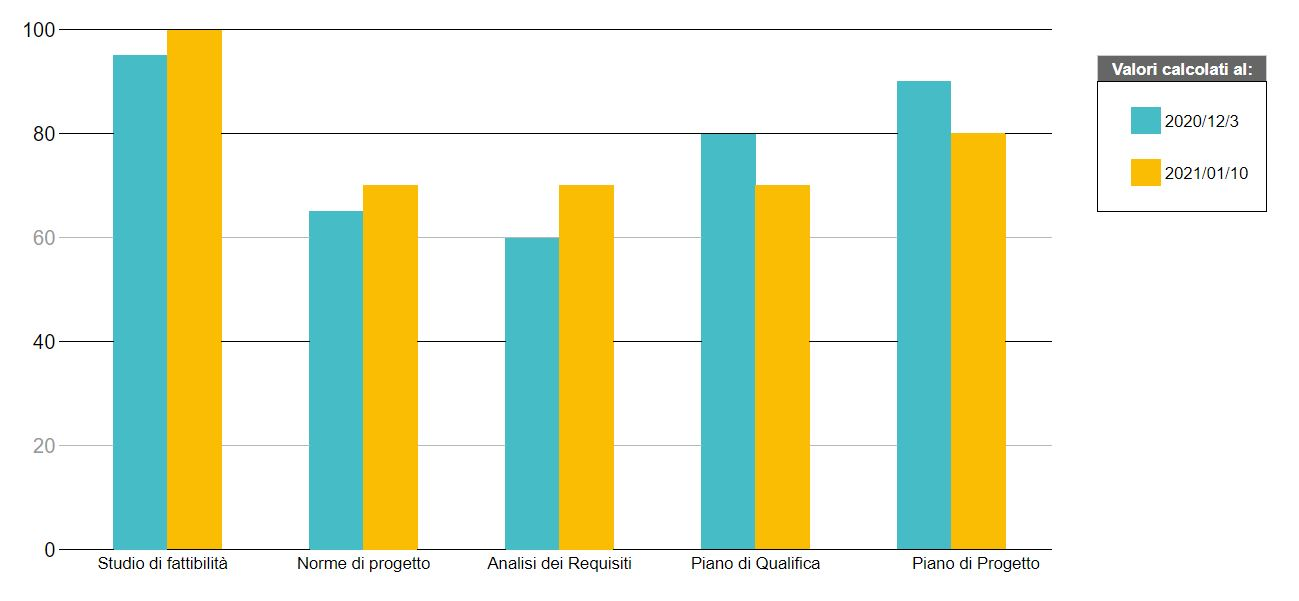
\includegraphics[width=15cm]{gulpeaseGrafico}
    \caption{Grafico dell'indice di Gulpease}
    \label{fig:img-valori-gulpease}
\end{figure}


\subsubsection{Errori ortografici}

Per quanto riguarda gli errori ortografici, oltre alla revisione fatta dai membri del gruppo, si è utilizzato anche lo spellchecker di Overleaf.


\subsection{Conclusioni}

In conclusione dai valori raggiunti dal grafico e dalla tabella soprastanti, si evince un discreto lavoro di redattori e verificatori. In particolare sono stati utili il Piano di Qualifica e le Norme di Progetto per avere un punto di riferimento, sia agli analisti nella scrittura dei documenti, sia ai verificatori per controllare con metriche e con parametri oggettivi.


    
\end{document}
